\documentclass{article}
\usepackage[utf8]{inputenc}
\usepackage{geometry}
\usepackage{amsmath}
\usepackage{amssymb}
\usepackage{enumitem}
\usepackage{graphicx}
\usepackage{multicol}
\usepackage{tikz}
\graphicspath{ {../images/} }

\geometry{letterpaper, margin=1in, portrait}

\begin{document}

\begin{center}
    {\LARGE EE114 - Homework 2} \\[0.5cm]
    Name: Kaushik Vada \\[0.5cm]
    \today
\end{center}

\section*{Problem 1.5.1}
Given the model of handoffs and call lengths in Problem 1.4.1,
\begin{enumerate}[label=(\alph*)]
    \item What is the probability that a brief call will have no handoffs? \\[1em]
    {\boldmath\textbf{$P[H_0 | B] = \frac{P[H_0 \cap B]}{P[B]} = \frac{0.4}{0.4 + 0.1 + 0.1} = \frac{0.4}{0.6} = \frac{2}{3} \approx 0.667$}}

    \item What is the probability that a call with one handoff will be long? \\[1em]
    {\boldmath\textbf{$P[L | H_1] = \frac{P[L \cap H_1]}{P[H_1]} = \frac{0.1}{0.1 + 0.1} = \frac{0.1}{0.2} = 0.5$}}

    \item What is the probability that a long call will have one or more handoffs? \\[1em]
    {\boldmath\textbf{$P[(H_1 \cup H_2) | L] = \frac{P[(H_1 \cup H_2) \cap L]}{P[L]} = \frac{P[H_1 \cap L] + P[H_2 \cap L]}{P[L]} = \frac{0.1 + 0.2}{0.1 + 0.1 + 0.2} = \frac{0.3}{0.4} = 0.75$}}
\end{enumerate}

\section*{Problem 1.5.3}
You have a shuffled deck of three cards: 2, 3, and 4. You draw one card. Let $C_i$ denote the event that card $i$ is picked. Let $E$ denote the event that card chosen is a even-numbered card.
\begin{enumerate}[label=(\alph*)]
    \item What is $P[C_2|E]$, the probability that the 2 is picked given that an even-numbered card is chosen? \\[1em]
    {\boldmath\textbf{The event $E$ (even card) is $\{2, 4\}$, so $P[E] = 2/3$. The intersection $C_2 \cap E$ is simply $\{2\}$, so $P[C_2 \cap E] = 1/3$.}} \\
    {\boldmath\textbf{$P[C_2|E] = \frac{P[C_2 \cap E]}{P[E]} = \frac{1/3}{2/3} = \frac{1}{2}$}}

    \item What is the conditional probability that an even-numbered card is picked given that the 2 is picked? \\[1em]
    {\boldmath\textbf{Given $C_2$ (card is 2), the card is definitely even, so $E \cap C_2 = \{2\}$ and $P[E \cap C_2] = 1/3$. Also $P[C_2] = 1/3$.}} \\
    {\boldmath\textbf{$P[E|C_2] = \frac{P[E \cap C_2]}{P[C_2]} = \frac{1/3}{1/3} = 1$}}
\end{enumerate}


\newpage

\section*{Problem 1.5.4}
From Problem 1.4.3, what is the conditional probability of $yy$, that a pea plant has two dominant genes given the event $Y$ that it has yellow seeds? \\[1em]
{\boldmath\textbf{From Problem 1.4.3, we have the following genotype probabilities:
\begin{itemize}
    \item $P[YY] = 1/4$ (Two dominant genes)
    \item $P[Yy] = 1/2$ (Hybrid)
    \item $P[yy] = 1/4$ (Two recessive genes)
\end{itemize}
The event $Y$ (yellow seeds) occurs for genotypes $\{YY, Yy\}$. The probability of $Y$ is:
\[ P[Y] = P[YY] + P[Yy] = 1/4 + 1/2 = 3/4 \]
We want to find the probability of having two dominant genes ($YY$) given $Y$. The intersection $\{YY\} \cap Y$ is simply $\{YY\}$, so $P[YY \cap Y] = 1/4$.
\[ P[YY | Y] = \frac{P[YY \cap Y]}{P[Y]} = \frac{1/4}{3/4} = \frac{1}{3} \]}}

\section*{Problem 1.6.1}
Is it possible for $A$ and $B$ to be independent events yet satisfy $A = B$? \\[1em]
{\boldmath\textbf{Yes, but only in trivial cases. \\
The definition of independence for events A and B is:
\[ P[A \cap B] = P[A]P[B] \]
If $A = B$, then $A \cap B = A \cap A = A$. The condition becomes:
\[ P[A] = P[A] \cdot P[A] = (P[A])^2 \]
Let $x = P[A]$. Then $x = x^2 \implies x^2 - x = 0 \implies x(x - 1) = 0$. \\
The solutions are $x = 0$ and $x = 1$. \\
Thus, $A$ and $B$ can be independent and equal if and only if $P[A] = 0$ or $P[A] = 1$.}}

\newpage

\section*{Problem 1.6.2}
Use a Venn diagram in which the event areas are proportional to their probabilities to illustrate two events $A$ and $B$ that are independent. \\[1em]
{\boldmath\textbf{We select probabilities $P[A]=0.4$ and $P[B]=0.5$. For independence, $P[A \cap B] = P[A]P[B] = 0.4 \times 0.5 = 0.2$. \\
This implies $P[A \cap B^c] = 0.4 - 0.2 = 0.2$ and $P[B \cap A^c] = 0.5 - 0.2 = 0.3$. \\
The area outside both events is $1 - (0.2+0.2+0.3) = 0.3$.
\begin{center}
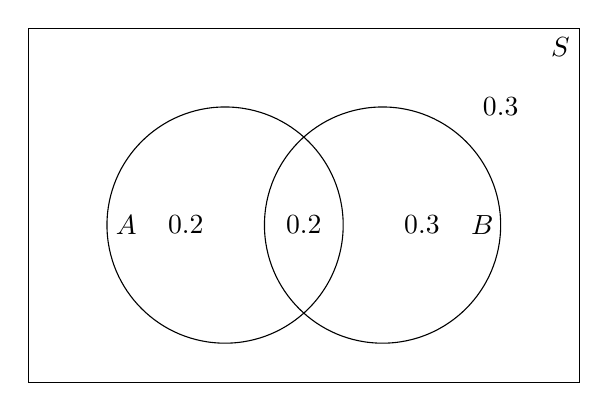
\begin{tikzpicture}
    \draw (0,0) circle (1.5cm) node[left=1cm] {$A$};
    \draw (2,0) circle (1.5cm) node[right=1cm] {$B$};
    \node at (1,0) {0.2};
    \node at (-0.5,0) {0.2};
    \node at (2.5,0) {0.3};
    \draw (-2.5,-2) rectangle (4.5,2.5) node[below left] {$S$};
    \node at (3.5,1.5) {0.3};
\end{tikzpicture}
\end{center}
Since the intersection area (0.2) equals the product of the individual probabilities ($0.4 \times 0.5$), the events $A$ and $B$ are visually independent.}}

\section*{Problem 1.6.3}
In an experiment, $A, B, C,$ and $D$ are events with probabilities $P[A] = 1/4$, $P[B] = 1/8$, $P[C] = 5/8$, and $P[D] = 3/8$. Furthermore, $A$ and $B$ are disjoint, while $C$ and $D$ are independent.
\begin{enumerate}[label=(\alph*)]
    \item Find $P[A \cap B]$, $P[A \cup B]$, $P[A \cap B^c]$, and $P[A \cup B^c]$. \\[1em]
    {\boldmath\textbf{Given $A, B$ are disjoint:
    \begin{itemize}
        \item $P[A \cap B] = 0$.
        \item $P[A \cup B] = P[A] + P[B] = 1/4 + 1/8 = 3/8$.
        \item $P[A \cap B^c] = P[A] = 1/4$ (Since $A$ and $B$ disjoint implies $A \subseteq B^c$).
        \item $P[A \cup B^c] = P(A) + P(B^c) - P(A \cap B^c) = 1/4 + (1 - 1/8) - 1/4 = 7/8$.
    \end{itemize}
    }}

    \item Are $A$ and $B$ independent? \\[1em]
    {\boldmath\textbf{No. Check: $P[A \cap B] = 0$. $P[A]P[B] = (1/4)(1/8) = 1/32$. \\
    Since $0 \neq 1/32$, they are not independent.}}

    \item Find $P[C \cap D]$, $P[C \cap D^c]$, and $P[C^c \cap D^c]$. \\[1em]
    {\boldmath\textbf{Given $C, D$ are independent:
    \begin{itemize}
        \item $P[C \cap D] = P[C]P[D] = (5/8)(3/8) = 15/64$.
        \item $P[C \cap D^c] = P[C]P[D^c] = (5/8)(1 - 3/8) = (5/8)(5/8) = 25/64$.
        \item $P[C^c \cap D^c] = P[C^c]P[D^c] = (1 - 5/8)(1 - 3/8) = (3/8)(5/8) = 15/64$.
    \end{itemize}
    }}

    \item Are $C^c$ and $D^c$ independent? \\[1em]
    {\boldmath\textbf{Yes. If $C$ and $D$ are independent, their complements are also independent. \\
    Verification: $P[C^c \cap D^c] = 15/64$. $P[C^c]P[D^c] = (3/8)(5/8) = 15/64$.}}
\end{enumerate}

\section*{Problem 1.6.4}
In an experiment, $A, B, C,$ and $D$ are events with probabilities $P[A \cup B] = 5/8$, $P[A] = 3/8$, $P[C \cap D] = 1/3$, and $P[C] = 1/2$. Furthermore, $A$ and $B$ are disjoint, while $C$ and $D$ are independent.
\begin{enumerate}[label=(\alph*)]
    \item Find $P[A \cap B]$, $P[B]$, $P[A \cap B^c]$, and $P[A \cup B^c]$. \\[1em]
    {\boldmath\textbf{Given $A, B$ are disjoint:
    \begin{itemize}
        \item $P[A \cap B] = 0$.
        \item $P[A \cup B] = P[A] + P[B] \implies 5/8 = 3/8 + P[B] \implies P[B] = 2/8 = 1/4$.
        \item $P[A \cap B^c] = P[A] = 3/8$ (Since $A \subseteq B^c$).
        \item $P[A \cup B^c] = P[A] + P[B^c] - P[A \cap B^c] = 3/8 + (1 - 1/4) - 3/8 = 3/4$.
    \end{itemize}
    }}

    \item Are $A$ and $B$ independent? \\[1em]
    {\boldmath\textbf{No. $P[A \cap B] = 0$, but $P[A]P[B] = (3/8)(1/4) = 3/32$. Since $0 \neq 3/32$, they are not independent.}}

    \item Find $P[D]$, $P[C \cap D^c]$, $P[C^c \cap D^c]$, and $P[C|D]$. \\[1em]
    {\boldmath\textbf{Given $C, D$ are independent:
    \begin{itemize}
        \item $P[C \cap D] = P[C]P[D] \implies 1/3 = (1/2)P[D] \implies P[D] = 2/3$.
        \item $P[C \cap D^c] = P[C]P[D^c] = (1/2)(1 - 2/3) = 1/6$.
        \item $P[C^c \cap D^c] = P[C^c]P[D^c] = (1 - 1/2)(1/3) = 1/6$.
        \item $P[C|D] = P(C) = 1/2$ (due to independence).
    \end{itemize}
    }}

    \item Find $P[C \cup D]$ and $P[C \cup D^c]$. \\[1em]
    {\boldmath\textbf{
    \begin{itemize}
        \item $P[C \cup D] = P[C] + P[D] - P[C \cap D] = 1/2 + 2/3 - 1/3 = 5/6$.
        \item $P[C \cup D^c] = P[C] + P[D^c] - P[C \cap D^c] = 1/2 + 1/3 - 1/6 = 4/6 = 2/3$.
    \end{itemize}
    }}

    \item Are $C$ and $D^c$ independent? \\[1em]
    {\boldmath\textbf{Yes. Since $C$ and $D$ are independent, $C$ and $D^c$ are also independent.}}
\end{enumerate}

\section*{Problem 1.6.5}
In an experiment with equiprobable outcomes, the event space is $S = \{1, 2, 3, 4\}$ and $P[s] = 1/4$ for all $s \in S$. Find three events in $S$ that are pairwise independent but are not independent. (Note: Pairwise independent events meet the first three conditions of Definition 1.8). \\[1em]
{\boldmath\textbf{Consider the events $A = \{1, 2\}$, $B = \{1, 3\}$, and $C = \{1, 4\}$.
\begin{itemize}
    \item $P[A] = P[B] = P[C] = 2/4 = 1/2$.
    \item $P[A \cap B] = P[\{1\}] = 1/4 = P[A]P[B]$. (Pairwise Independent)
    \item $P[A \cap C] = P[\{1\}] = 1/4 = P[A]P[C]$. (Pairwise Independent)
    \item $P[B \cap C] = P[\{1\}] = 1/4 = P[B]P[C]$. (Pairwise Independent)
\end{itemize}
Check mutual independence:
\[ P[A \cap B \cap C] = P[\{1\}] = 1/4 \]
\[ P[A]P[B]P[C] = (1/2)^3 = 1/8 \]
Since $1/4 \neq 1/8$, the events are pairwise independent but not mutually independent.}}

\section*{Problem 1.6.7}
For independent events $A$ and $B$, prove that
\begin{enumerate}[label=(\alph*)]
    \item $A$ and $B^c$ are independent. \\[1em]
    {\boldmath\textbf{We need to show $P[A \cap B^c] = P[A]P[B^c]$.
    \begin{align*}
        P[A] &= P[A \cap B] + P[A \cap B^c] \quad \text{(Total Probability)} \\
        P[A \cap B^c] &= P[A] - P[A \cap B] \\
        &= P[A] - P[A]P[B] \quad \text{(Since A, B independent)} \\
        &= P[A](1 - P[B]) \\
        &= P[A]P[B^c]. \quad \text{(Proven)}
    \end{align*}
    }}

    \item $A^c$ and $B$ are independent. \\[1em]
    {\boldmath\textbf{We need to show $P[A^c \cap B] = P[A^c]P[B]$.
    \begin{align*}
        P[B] &= P[A \cap B] + P[A^c \cap B] \\
        P[A^c \cap B] &= P[B] - P[A \cap B] \\
        &= P[B] - P[A]P[B] \quad \text{(Since A, B independent)} \\
        &= P[B](1 - P[A]) \\
        &= P[B]P[A^c]. \quad \text{(Proven)}
    \end{align*}
    }}

    \item $A^c$ and $B^c$ are independent. \\[1em]
    {\boldmath\textbf{We need to show $P[A^c \cap B^c] = P[A^c]P[B^c]$.
    \begin{align*}
        P[A^c \cap B^c] &= P[(A \cup B)^c] \quad \text{(De Morgan's Law)} \\
        &= 1 - P[A \cup B] \\
        &= 1 - (P[A] + P[B] - P[A \cap B]) \\
        &= 1 - P[A] - P[B] + P[A]P[B] \quad \text{(Independence)} \\
        &= (1 - P[A]) - P[B](1 - P[A]) \\
        &= (1 - P[A])(1 - P[B]) \\
        &= P[A^c]P[B^c]. \quad \text{(Proven)}
    \end{align*}
    }}
\end{enumerate}

\end{document}
